\section{Results}

We train on 10000 simulated worlds with star objects of variable size placed at
random positions with random orientations. We enforce that no two objects are
within \unit{3}{\m} of each other. We build our observation model from simulated
LIDAR scans from these worlds and the ground truth position and orientation of
the objects.

Then, we generate a LIDAR scan from an unseen simulated world. This is shown in
\figref{fig:sim_world}. We run our detector on this LIDAR data. Because of the
symmetry of the star, we test only orientations between $\unit{0}{\degree}$ and
$\unit{72}{\degree}$. The result of the detector is shown in
\figref{fig:detector}.
%
\begin{figure}
  \centering
  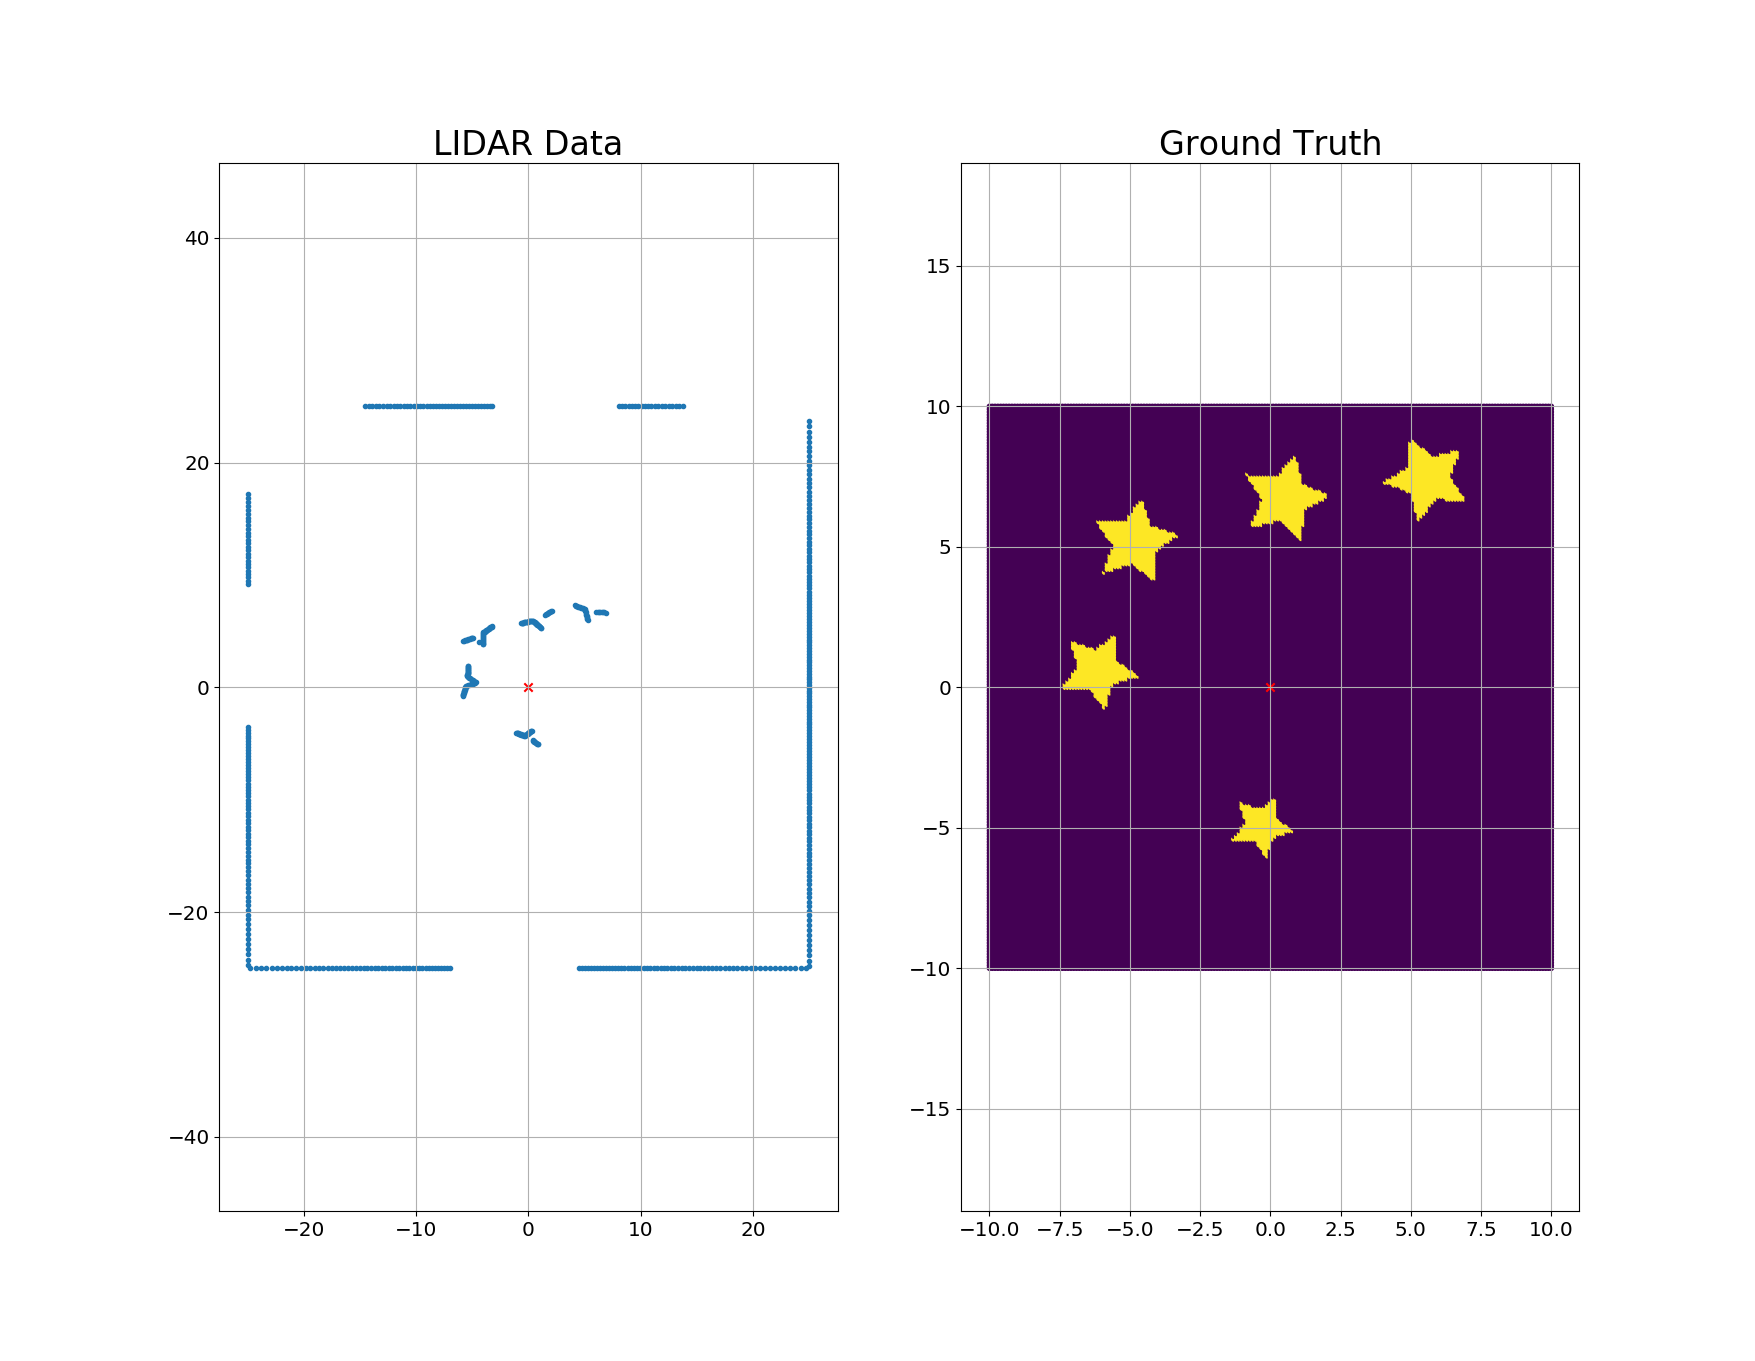
\includegraphics[width=\columnwidth]{figures/ground_truth.png}
  \caption{Simulation. On the left is the simular LIDAR scan of the environment.
    The right figure depicts the ground truth position of all objects in the
    scene.}
  \label{fig:sim_world}
\end{figure}
%
\begin{figure*}
  \centering
  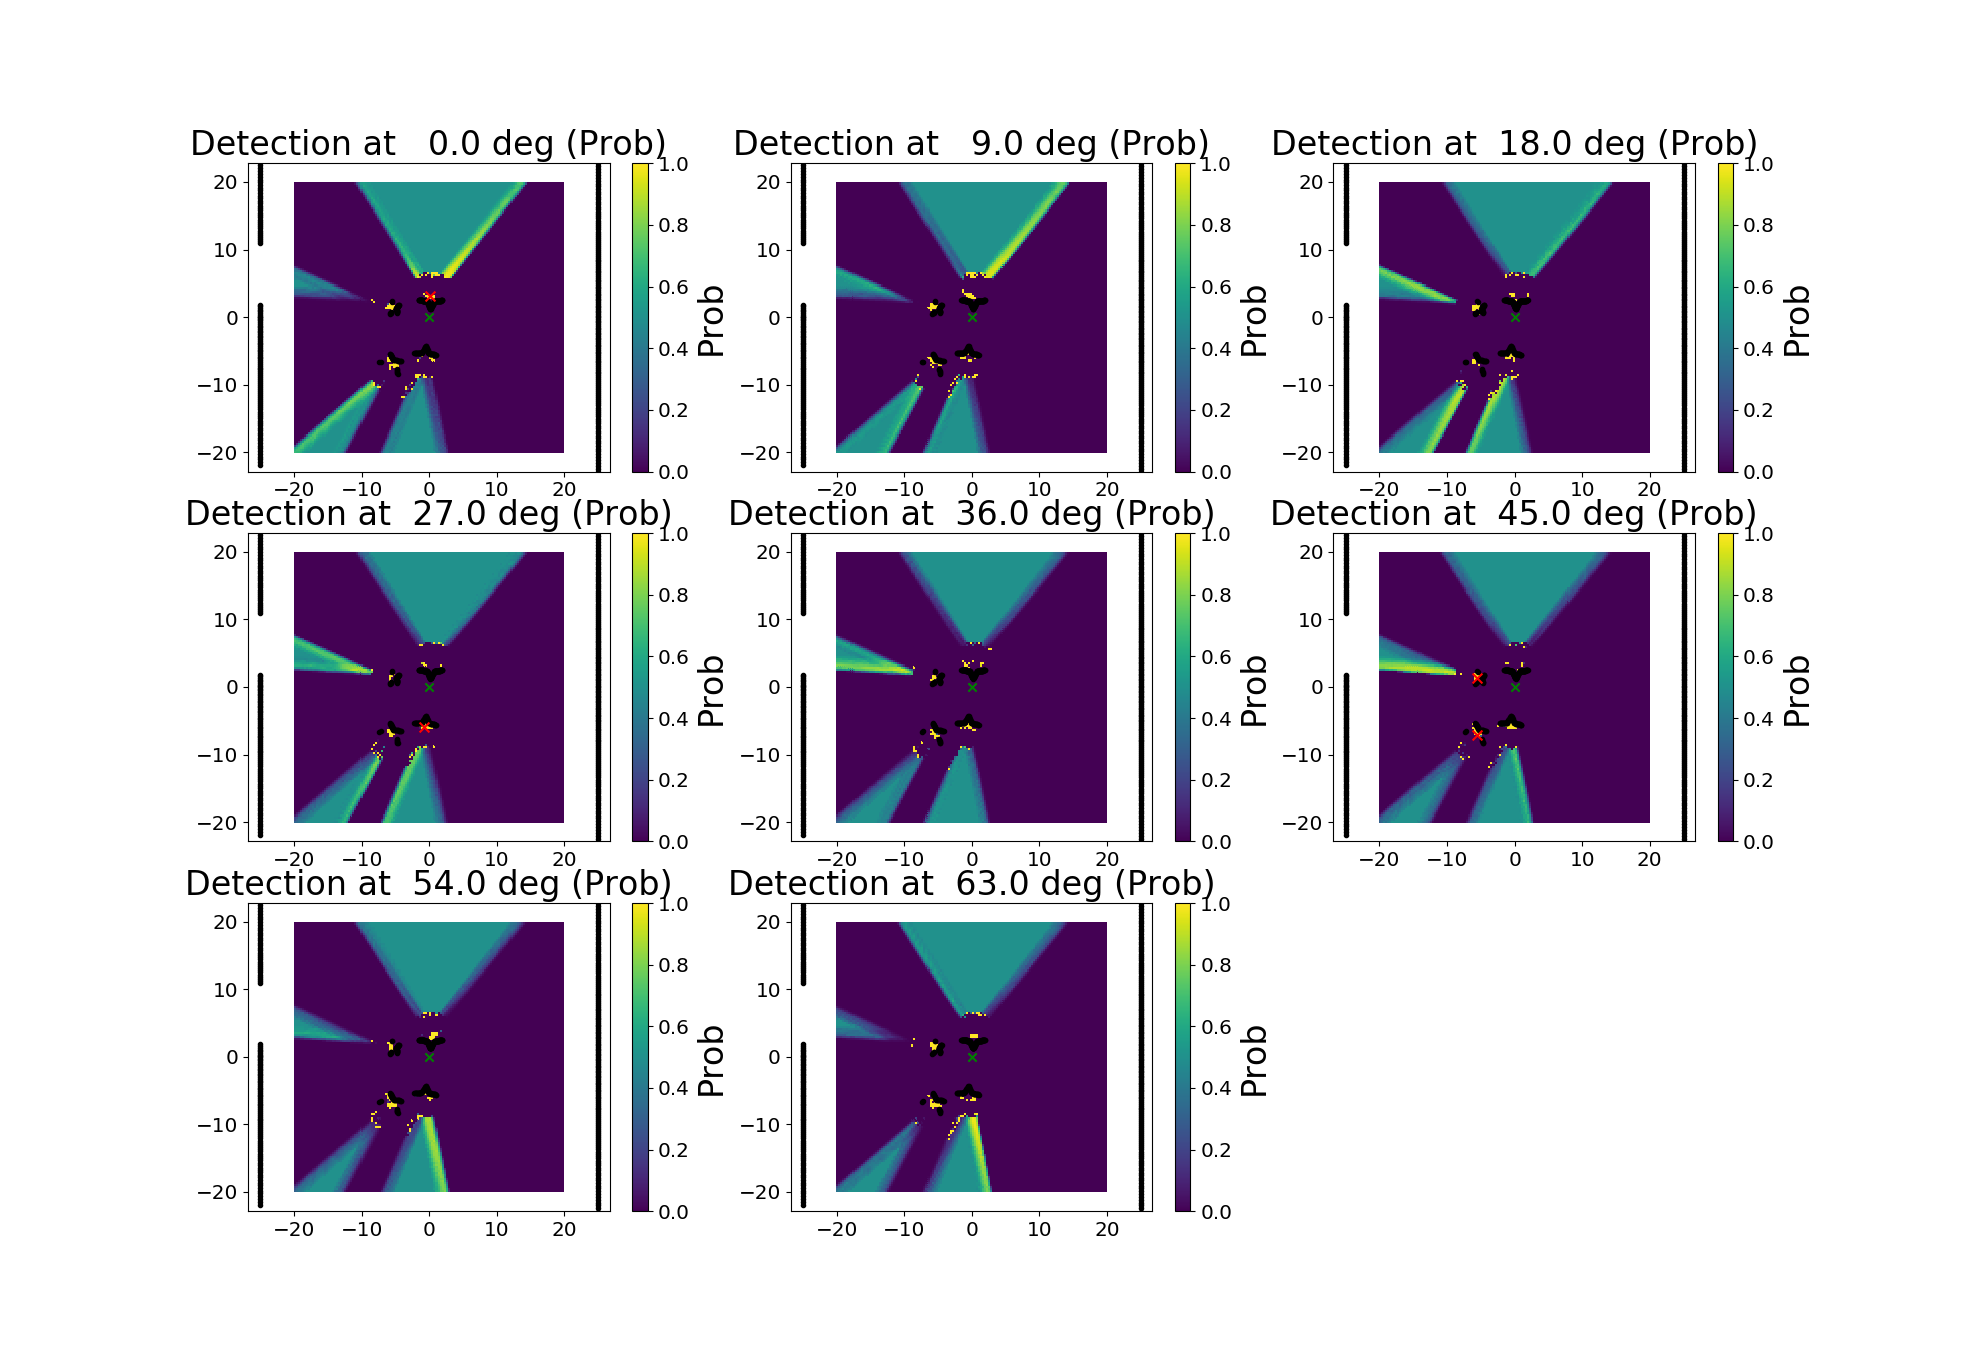
\includegraphics[width=\textwidth]{figures/detections.png}
  \caption{Result of detector. Non-maximal suppression results in detections
    marked with red x's}
  \label{fig:detector}
\end{figure*}


